\documentclass[a4paper,12pt]{article}

\usepackage[T2A]{fontenc}
\usepackage[utf8]{inputenc}
\usepackage[russian]{babel}
\usepackage{graphicx}
\usepackage{geometry}
\usepackage{listings}
\usepackage{xcolor}
\usepackage{float}
\usepackage{setspace}

\geometry{left=2cm,right=2cm,top=2cm,bottom=2cm}

\lstset{
  language=C++,
  basicstyle=\ttfamily\footnotesize\setstretch{0.82},
  keywordstyle=\color{blue},
  commentstyle=\color{gray},
  stringstyle=\color{teal},
  numbers=left,
  numberstyle=\tiny\color{gray},
  stepnumber=1,
  numbersep=6pt,
  tabsize=2,
  breaklines=true,
  frame=single,
  framerule=0.3pt,
  framesep=3pt,
  aboveskip=6pt,
  belowskip=6pt,
  lineskip=-1pt,
  showstringspaces=false
}

\begin{document}

\begin{center}
  {\Large Отчет по блоку 4}\\
  \vspace{0.5cm}
  {\large Алгоритмы и структуры данных}
\end{center}

\tableofcontents
\newpage

\section{Задача M}

\subsection*{Текст задания}
\begin{figure}[H]
  \centering
  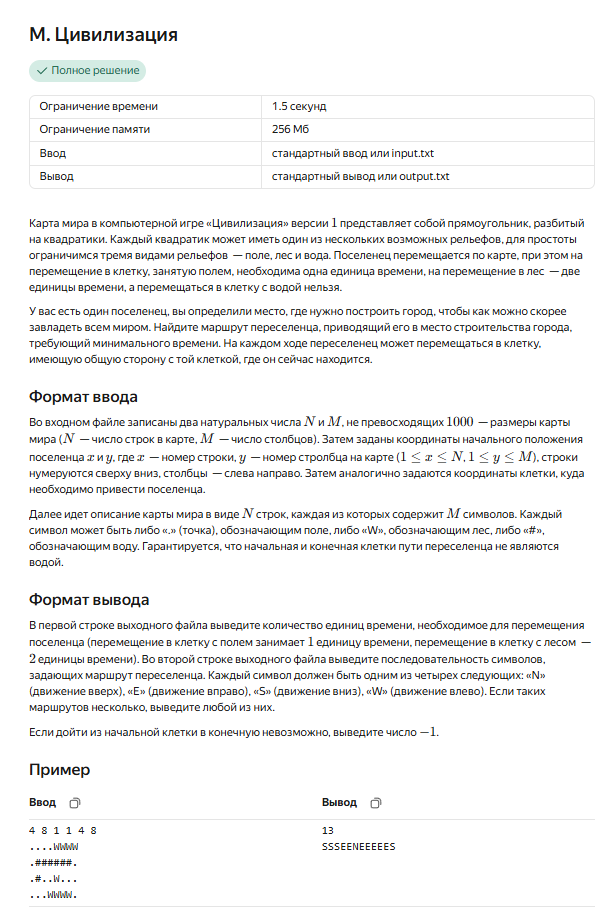
\includegraphics[width=\textwidth,height=0.78\textheight,keepaspectratio]{task_m/task.png}
\end{figure}

\subsection*{Пояснение к алгоритму}
Карта представляется как граф, где каждая свободная клетка является вершиной. Из клетки можно перейти в соседние по стороне клетки, если там нет стены. Стоимость перехода зависит от типа клетки: обычная клетка стоит 1, а клетка с водой стоит 2. Для поиска минимальной стоимости пути используется алгоритм Дейкстры, потому что все веса переходов положительные. Чтобы восстановить маршрут, для каждой клетки запоминается предыдущая клетка в кратчайшем пути.

\subsection*{Сложность по времени}
$O(nm \log(nm))$, где $n$ и $m$ - размеры поля.

\subsection*{Сложность по памяти}
$O(nm)$.

\subsection*{Код}
\lstinputlisting{task_m/m.cpp}

\newpage
\section{Задача N}

\subsection*{Текст задания}
\begin{figure}[H]
  \centering
  
\includegraphics[width=\textwidth,height=0.78\textheight,keepaspectratio]{task_n/task.png}
\end{figure}

\subsection*{Пояснение к алгоритму}
Каждое число задает переход из одной вершины в другую, поэтому получается функциональный граф. Нужно посчитать количество циклов в таком графе. Для этого запускается обход из каждой еще не посещенной вершины. В массиве посещений хранится номер старта текущего обхода. Если обход пришел в вершину, которая уже была посещена в этом же запуске, значит найден новый цикл.

\subsection*{Сложность по времени}
$O(n)$.

\subsection*{Сложность по памяти}
$O(n)$.

\subsection*{Код}
\lstinputlisting{task_n/n.cpp}

\newpage
\section{Задача O}

\subsection*{Текст задания}
\begin{figure}[H]
  \centering
  
\includegraphics[width=\textwidth,height=0.78\textheight,keepaspectratio]{task_o/task.png}
\end{figure}

\subsection*{Пояснение к алгоритму}
Граф проверяется на двудольность. Для этого каждой вершине пытаемся назначить один из двух цветов. Обход в ширину раскрашивает соседей в противоположный цвет. Если во время обхода находится ребро между вершинами одного цвета, то граф не является двудольным. Так как граф может быть несвязным, обход запускается из каждой еще не раскрашенной вершины.

\subsection*{Сложность по времени}
$O(n + m)$, где $n$ - количество вершин, а $m$ - количество ребер.

\subsection*{Сложность по памяти}
$O(n + m)$.

\subsection*{Код}
\lstinputlisting{task_o/o.cpp}

\newpage
\section{Задача P}

\subsection*{Текст задания}
\begin{figure}[H]
  \centering
  
\includegraphics[width=\textwidth,height=0.6\textheight,keepaspectratio]{task_p/task.png}
\end{figure}

\subsection*{Пояснение к алгоритму}
Нужно найти минимальное значение ограничения, при котором граф становится сильно связным. Для фиксированного значения оставляются только ребра с весом не больше этого значения. Затем проверяется достижимость всех вершин из первой вершины и достижимость первой вершины из всех остальных с помощью обхода в обратном графе. Если обе проверки успешны, граф сильно связен при этом ограничении. Ответ ищется бинарным поиском по возможному значению ограничения.

\subsection*{Сложность по времени}
$O(n^2 \log C)$, где $n$ - количество вершин, а $C$ - диапазон значений весов.

\subsection*{Сложность по памяти}
$O(n^2)$.

\subsection*{Код}
\lstinputlisting{task_p/p.cpp}

\end{document}
